\begin{figure*}[ht]
    \centering
    \vspace{-3mm}
    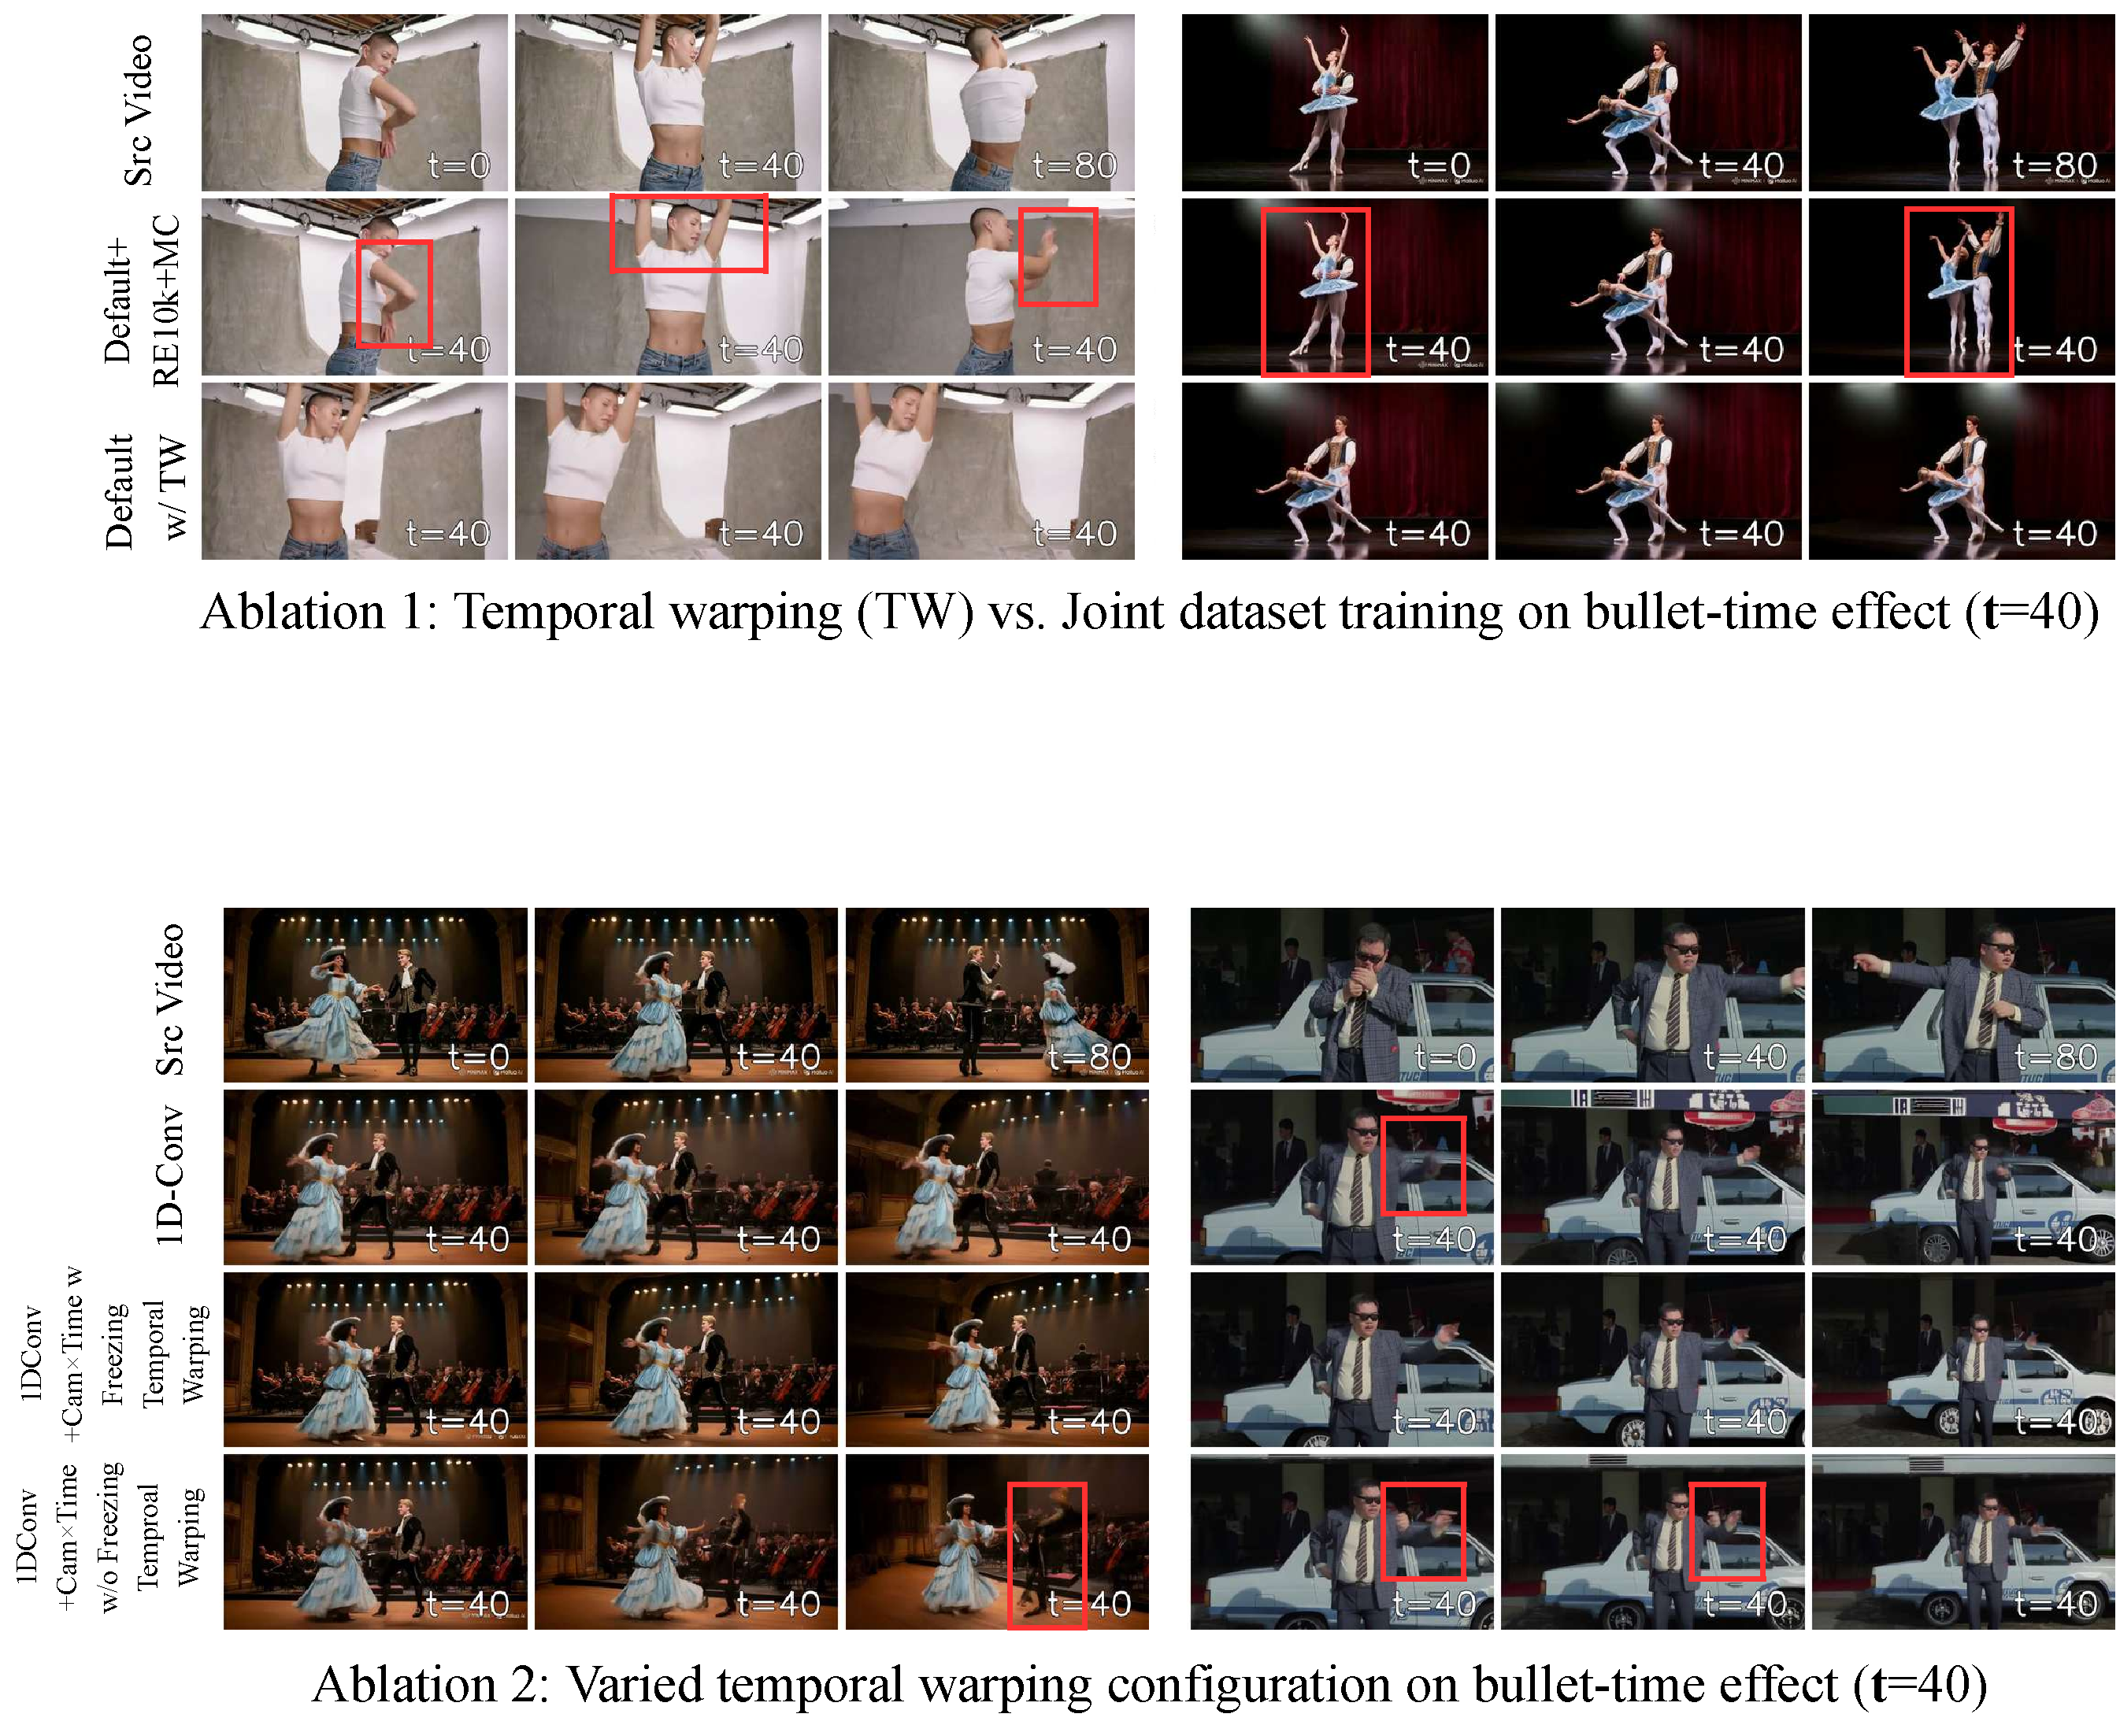
\includegraphics[width=\linewidth]{figures/src_files/ablation_1_2.pdf}
    
    \caption{
    \textbf{Ablation study.}
    (Top) Using \cite{Bai2025,bai2024syncammaster} as default datasets, we compare the influence of adding static-scene datasets \cite{zhou2018stereo,li2019mannequin} vs.~just doing temporal warping (TW) augmentation (Sec.~3.2.2 in the main paper). Temporal warping definitely provide more variety of time control signals, allowing models to learn better camera-time disentanglement. 
    (Bottom) We further compare different configurations of warping, where we show freezing temporal warping (3\textsuperscript{rd} row) leads to better results than those trained without freezing temporal warping.
    }
    \label{fig:ablation_1_2}
\end{figure*}
